%%%%%%%%%%%%%%%%%%%%%%%%%%%%%%%%%%%%%%%%%%%%%%%%%%%%%%%
% A template for Wiley article submissions to Networks.
% Developed by Overleaf.
%
% Modified by D. Shier  (13 Feb 2019)
%%
% Usage notes:
% % Use "num-refs" option for numerical citation and references style.
% % Use the attached wiley-networks.cls and abbrv_networks.bst files.

\documentclass[num-refs]{wiley-networks}

% Add additional packages here if required


% Update article type if known
\papertype{Yellow Paper}
\paperfield{DRAFT: Version 0.1} 

\title{Qredo Custody Network}

% Use the \authfn to add symbols for additional footnotes and present addresses, if any. Usually start with 1 for notes about author contributions; then continuing with 2 etc if any author has a different present address.

\author[1\authfn{1}]{Dr. Kealan McCusker}
\author[2\authfn{1}]{Brian Spector}

\contrib[\authfn{1}]{With assistance from Qredo Ltd staff and other Apache Milagro contributors.}

% Include full affiliation details for all authors
\affil[1]{PPMC Member and Contributor to Apache Milagro, Chief Cryptographer at Qredo Ltd}
\affil[2]{PPMC Member and Contributor to Apache Milagro, Chief Product and Strategy Officer at Qredo Ltd}

\corraddress{Qredo Ltd, 1 Primrose Street, London, UK, EC4R 1AG}

\corremail{info@qredo.com}

\begin{document}

\maketitle

\begin{abstract}
The Qredo Custody Network is a decentralized paradigm for digital asset custody. Qredo's network makes use of cryptographic libraries and applications from Apache Milagro, an open source software project hosted at the Apache Software Foundation, the largest open source software foundation globally. Much of the content for this paper is sourced directly from the Apache Milagro website. We encourage the reader to visit https://milagro.apache.org to get involved in the project directly.
\end{abstract}

\section{Introduction}
Digital asset custody in its current form is fundamentally broken. The centralization of asset storage by cold storage custodians has introduced a drag on cryptocurrency adoption by large fiduciary institutional investors. 

Central to this issue are an inability to naturally segregate custodial wallets to an individual level, no visibility over custodian operations, co-mingling of customer funds, and an inability to redeem assets to beneficiaries in near real-time to take advantage of market trading opportunities.

\subsection{Sector Irony}
The irony of the situation is that by centralizing custodial operations to cold storage vendors, the industry has retarded its growth prospects with the largest fiduciary institutional investors who have the ability to take cryptocurrency adoption into the mainstream. However, if the concepts of decentralization are applied to custodial operations over digital assets, then the requirements that large fiduciary institutional investors have can be met.

\subsection{A New Approach: Decentralized Custody}
The Qredo Custody Network is a decentralized approach to digital asset custody. It works by creating a decentralized network of clients, called Fiduciaries, who work in coordinated yet graduated steps to obtain digital signatures over messages. Fiduciaries can act as Master Fiduciaries, organizing other Fiduciaries and then combine these signatures into a complete group signature based on thresholds set by the originating Principal. 

Qredo Ltd acts as a Master Fiduciary can also act as signature combiner service, operated by Qredo Ltd, The final signature being used to create a transient secret key that, when cryptographically combined with other secret keys, will reveal the private key to control assets within a custodial wallet, thereby controlling the assets placed into the wallet. 





\section{Imagine the blockchain as a custodian}

% Equations should be inserted using standard LaTeX equation and eqnarray environments, not as graphics, and should be set in the main text
This is an equation, numbered
\begin{equation}
\int_0^{+\infty}e^{-x^2}dx=\frac{\sqrt{\pi}}{2},
\end{equation}
as well as on one that is not numbered
\begin{equation*}
e^{i\pi}=-1
\end{equation*}

We can also have multiline expressions, as shown next:
\begin{eqnarray*}
x_1&= & [w(1,2) + w(1,2) x_2] + [w(1,3) + w(1,3) x_3] + [w(1,4) + w(1,4) x_4] \\
      &= & w(1,2) [1+ x_2] + w(1,3)[1 + x_3] + w(1,4)[1  +  x_4] \\
      &= & \tfrac{1}{3} [1+ x_2] + \tfrac{1}{3}[1 + x_3] + \tfrac{1}{3}[1  +  x_4] .
\end{eqnarray*}

Below we display a transition matrix $A$:
\[
A = \begin{bmatrix}
0 & 0 & 0 & 1\\
\frac{1}{4} & 0 & \frac{3}{4} & 0\\[.06cm]
\frac{1}{2} & 0 & 0 & \frac{1}{2}\\[.05cm]
0 & 1 & 0 & 0
       \end{bmatrix}.
\]




\subsection{Adding Citations and a References List}

Please use a \verb|.bib| file to store your references. Just remember to specify the filename of the \verb|.bib|.

Citations should use the reference list style provided in the  abbrv$\_$networks.bst file. You can then cite entries from it, like this: \cite{Adams}. 


Additional work is found in the books \cite{AhujaEtal, vonNeumann}, works appearing as book chapters \cite{ReadTutte, Shapiro}, articles in proceedings \cite{Goemans, Seibert}, technical reports \cite{Jones}, and in theses \cite{Ponza, Wilson}.





\subsubsection{Third Level Heading}
Figures and tables are numbered with Arabic numerals and are placed near their occurrence in the text of the article. 
Figures should contain a caption displayed underneath.
Tables should be self-contained and complement, but not duplicate, information contained in the text. They should be not be provided as images. Legends should be concise but comprehensive. The table, legend, and footnotes must be understandable without reference to the text.

Appendices will be placed after the references. 

\begin{figure}[h!]
\centering
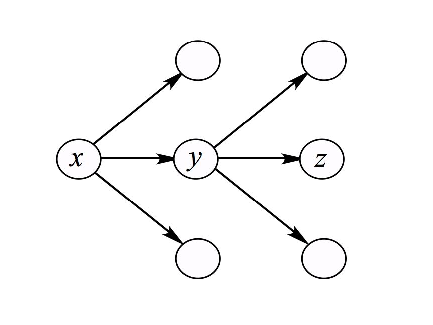
\includegraphics[width=120pt]{figure2aa}
\caption{A sample figure.}
\end{figure}

\begin{table}[h]
\caption{This is a table. }
\begin{threeparttable}
\begin{tabular}{lccrr}
\headrow
\thead{Variables} & \thead{JKL ($\boldsymbol{n=30}$)} & \thead{Control ($\boldsymbol{n=40}$)} & \thead{MN} & \thead{$\boldsymbol t$ (68)}\\
Age at testing & 38 & 58 & 504.48 & 58 ms\\
Age at testing & 38 & 58 & 504.48 & 58 ms\\
Age at testing & 38 & 58 & 504.48 & 58 ms\\
Age at testing & 38 & 58 & 504.48 & 58 ms\\
\hiderowcolors
stop alternating row colors from here onwards\\
Age at testing & 38 & 58 & 504.48 & 58 ms\\
Age at testing & 38 & 58 & 504.48 & 58 ms\\
\hline  % Please only put a hline at the end of the table
\end{tabular}

\begin{tablenotes}
\item JKL, just keep laughing; MN, merry noise.
\end{tablenotes}
\end{threeparttable}
\end{table}



\paragraph{Fourth Level Heading}
Here are examples of a quote

\begin{quote}
The significant problems we have cannot be solved at the same level of thinking with which we created them.
\end{quote}

\noindent and an epigraph

\begin{epigraph}{Albert Einstein}
Anyone who has never made a mistake has never tried anything new.
\end{epigraph}

\section{Imagine the blockchain as a custodian}

\section*{\normalsize{ACKNOWLEDGMENTS}}
Acknowledgments should include contributions from anyone who does not meet the criteria for authorship (for example, to recognize contributions from people who provided technical help, collation of data, writing assistance, acquisition of funding, or a department chairperson who provided general support), as well as any funding or other support information.

%REFERENCES
%Note that references are placed in lexicographic order by author name. Multiple entries within a citation should appear in numerical order also, such as [2, 17, 19, 42].

%\bibliographystyle{plain}
\bibliography{sample}

\end{document} 